% Options for packages loaded elsewhere
% Options for packages loaded elsewhere
\PassOptionsToPackage{unicode}{hyperref}
\PassOptionsToPackage{hyphens}{url}
%
\documentclass[
  ignorenonframetext,
  aspectratio=169,
  russian,
]{beamer}
\newif\ifbibliography
\usepackage{pgfpages}
\setbeamertemplate{caption}[numbered]
\setbeamertemplate{caption label separator}{: }
\setbeamercolor{caption name}{fg=normal text.fg}
\beamertemplatenavigationsymbolsempty
% remove section numbering
\setbeamertemplate{part page}{
  \centering
  \begin{beamercolorbox}[sep=16pt,center]{part title}
    \usebeamerfont{part title}\insertpart\par
  \end{beamercolorbox}
}
\setbeamertemplate{section page}{
  \centering
  \begin{beamercolorbox}[sep=12pt,center]{section title}
    \usebeamerfont{section title}\insertsection\par
  \end{beamercolorbox}
}
\setbeamertemplate{subsection page}{
  \centering
  \begin{beamercolorbox}[sep=8pt,center]{subsection title}
    \usebeamerfont{subsection title}\insertsubsection\par
  \end{beamercolorbox}
}
% Prevent slide breaks in the middle of a paragraph
\widowpenalties 1 10000
\raggedbottom
\AtBeginPart{
  \frame{\partpage}
}
\AtBeginSection{
  \ifbibliography
  \else
    \frame{\sectionpage}
  \fi
}
\AtBeginSubsection{
  \frame{\subsectionpage}
}
\usepackage{iftex}
\ifPDFTeX
  \usepackage[T1]{fontenc}
  \usepackage[utf8]{inputenc}
  \usepackage{textcomp} % provide euro and other symbols
\else % if luatex or xetex
  \usepackage{unicode-math} % this also loads fontspec
  \defaultfontfeatures{Scale=MatchLowercase}
  \defaultfontfeatures[\rmfamily]{Ligatures=TeX,Scale=1}
\fi
\usepackage{lmodern}

\usetheme[]{Madrid}
\usefonttheme{serif} % use mainfont rather than sansfont for slide text
\ifPDFTeX\else
  % xetex/luatex font selection
  \setmainfont[]{DejaVu Sans}
  \setsansfont[]{DejaVu Sans}
  \setmathfont[]{DejaVu Sans}
\fi
% Use upquote if available, for straight quotes in verbatim environments
\IfFileExists{upquote.sty}{\usepackage{upquote}}{}
\IfFileExists{microtype.sty}{% use microtype if available
  \usepackage[]{microtype}
  \UseMicrotypeSet[protrusion]{basicmath} % disable protrusion for tt fonts
}{}
\makeatletter
\@ifundefined{KOMAClassName}{% if non-KOMA class
  \IfFileExists{parskip.sty}{%
    \usepackage{parskip}
  }{% else
    \setlength{\parindent}{0pt}
    \setlength{\parskip}{6pt plus 2pt minus 1pt}}
}{% if KOMA class
  \KOMAoptions{parskip=half}}
\makeatother


\usepackage{longtable,booktabs,array}
\usepackage{calc} % for calculating minipage widths
\usepackage{caption}
% Make caption package work with longtable
\makeatletter
\def\fnum@table{\tablename~\thetable}
\makeatother
\usepackage{graphicx}
\makeatletter
\newsavebox\pandoc@box
\newcommand*\pandocbounded[1]{% scales image to fit in text height/width
  \sbox\pandoc@box{#1}%
  \Gscale@div\@tempa{\textheight}{\dimexpr\ht\pandoc@box+\dp\pandoc@box\relax}%
  \Gscale@div\@tempb{\linewidth}{\wd\pandoc@box}%
  \ifdim\@tempb\p@<\@tempa\p@\let\@tempa\@tempb\fi% select the smaller of both
  \ifdim\@tempa\p@<\p@\scalebox{\@tempa}{\usebox\pandoc@box}%
  \else\usebox{\pandoc@box}%
  \fi%
}
% Set default figure placement to htbp
\def\fps@figure{htbp}
\makeatother



\ifLuaTeX
\usepackage[bidi=basic,provide=*]{babel}
\else
\usepackage[bidi=default,provide=*]{babel}
\fi
\ifPDFTeX
\else
\babelfont{rm}[]{DejaVu Sans}
\fi
% get rid of language-specific shorthands (see #6817):
\let\LanguageShortHands\languageshorthands
\def\languageshorthands#1{}


\setlength{\emergencystretch}{3em} % prevent overfull lines

\providecommand{\tightlist}{%
  \setlength{\itemsep}{0pt}\setlength{\parskip}{0pt}}



 


\IfFileExists{plex-otf.sty}{
  %% Full TeXlive
  % \usepackage[%
  %   % math,
  %   RM={Scale=0.94},SS={Scale=0.94},SScon={Scale=0.94},TT={Scale=MatchLowercase,FakeStretch=0.9},DefaultFeatures={Ligatures=Common}
  % ]{plex-otf}
}{
  %% TinyTeX
  \usepackage{libertine}
}

%%% Load theme
% https://deic.uab.cat/~iblanes/beamer_gallery/
\IfFileExists{beamerthemegotham.sty}{
  %% Full TeXlive
  \usetheme{gotham}
  \gothamset{
    numbering=totalpagenumber,
    parttocframe default=off,
    sectiontocframe default=off,
    subsectiontocframe default=off,
  }
}{
  %% TinyTeX
  \usetheme{Madrid}
}
\makeatletter
\@ifpackageloaded{caption}{}{\usepackage{caption}}
\AtBeginDocument{%
\ifdefined\contentsname
  \renewcommand*\contentsname{Содержание}
\else
  \newcommand\contentsname{Содержание}
\fi
\ifdefined\listfigurename
  \renewcommand*\listfigurename{Список иллюстраций}
\else
  \newcommand\listfigurename{Список иллюстраций}
\fi
\ifdefined\listtablename
  \renewcommand*\listtablename{Список таблиц}
\else
  \newcommand\listtablename{Список таблиц}
\fi
\ifdefined\figurename
  \renewcommand*\figurename{Рисунок}
\else
  \newcommand\figurename{Рисунок}
\fi
\ifdefined\tablename
  \renewcommand*\tablename{Таблица}
\else
  \newcommand\tablename{Таблица}
\fi
}
\@ifpackageloaded{float}{}{\usepackage{float}}
\floatstyle{ruled}
\@ifundefined{c@chapter}{\newfloat{codelisting}{h}{lop}}{\newfloat{codelisting}{h}{lop}[chapter]}
\floatname{codelisting}{Список}
\newcommand*\listoflistings{\listof{codelisting}{Листинги}}
\makeatother
\makeatletter
\makeatother
\makeatletter
\@ifpackageloaded{caption}{}{\usepackage{caption}}
\@ifpackageloaded{subcaption}{}{\usepackage{subcaption}}
\makeatother

\usepackage{bookmark}
\IfFileExists{xurl.sty}{\usepackage{xurl}}{} % add URL line breaks if available
\urlstyle{same}
\hypersetup{
  pdftitle={Отчет по лабораторной работе №5},
  pdfauthor={Богомолова Полина Петровна},
  pdflang={ru},
  hidelinks,
  pdfcreator={LaTeX via pandoc}}


\title{Отчет по лабораторной работе №5}
\subtitle{Настройка рабочей среды}
\author{Богомолова Полина Петровна}
\date{2026-04-16}

\begin{document}
\frame{\titlepage}

\renewcommand*\contentsname{Содержание}
\begin{frame}[allowframebreaks]
  \frametitle{Содержание}
  \setcounter{tocdepth}{1}
  \tableofcontents
\end{frame}
\setcounter{tocdepth}{1}
\tableofcontents
}

\begin{frame}{Информация о докладчике}
\phantomsection\label{ux438ux43dux444ux43eux440ux43cux430ux446ux438ux44f-ux43e-ux434ux43eux43aux43bux430ux434ux447ux438ux43aux435}
Богомолова Полина Петровна, ФФМиЕН, НКАбд01-25, 1032253562 ---
\end{frame}

\begin{frame}{Цель работы}
\phantomsection\label{ux446ux435ux43bux44c-ux440ux430ux431ux43eux442ux44b}
Установить менеджеры паролей pass и gopass.\\
Освоить работу с ними.\\
Настроить интеграцию с браузером.\\
Научиться синхронизировать конфигурации между машинами с помощью
chezmoi.
\end{frame}

\begin{frame}{Задание}
\phantomsection\label{ux437ux430ux434ux430ux43dux438ux435}
Установить pass и gopass\\
Просмотреть список gpg ключей\\
Инициализировать хранилище\\
Синхронизировать с git\\
Настроить интерфейс браузера\\
Создать и сгенерировать пароль\\
Использовать chezmoi на нескольких машинах
\end{frame}

\begin{frame}{Теоретическое введение}
\phantomsection\label{ux442ux435ux43eux440ux435ux442ux438ux447ux435ux441ux43aux43eux435-ux432ux432ux435ux434ux435ux43dux438ux435}
pass --- стандартный менеджер паролей для Unix.\\
Пароли хранятся в файловой системе и шифруются с помощью GPG.

gopass --- расширенная реализация pass на языке Go.

chezmoi --- инструмент для управления конфигурационными файлами и
синхронизации между машинами.
\end{frame}

\begin{frame}{Установка pass}
\phantomsection\label{ux443ux441ux442ux430ux43dux43eux432ux43aux430-pass}
\begin{figure}

\centering{


\includegraphics[width=0.5\linewidth,height=\textheight,keepaspectratio]{image/1.png}

}

\caption{\label{fig-001}Рисунок 1 --- Установка pass}

\end{figure}%
\end{frame}

\begin{frame}{Проверка установки pass}
\phantomsection\label{ux43fux440ux43eux432ux435ux440ux43aux430-ux443ux441ux442ux430ux43dux43eux432ux43aux438-pass}
\begin{figure}

\centering{


\includegraphics[width=0.5\linewidth,height=\textheight,keepaspectratio]{image/2.png}

}

\caption{\label{fig-002}Рисунок 2 --- Проверка установки pass}

\end{figure}%
\end{frame}

\begin{frame}{Установка gopass}
\phantomsection\label{ux443ux441ux442ux430ux43dux43eux432ux43aux430-gopass}
\begin{figure}

\centering{


\includegraphics[width=0.5\linewidth,height=\textheight,keepaspectratio]{image/3.png}

}

\caption{\label{fig-003}Рисунок 3 --- Установка gopass}

\end{figure}%
\end{frame}

\begin{frame}{Проверка установки gopass}
\phantomsection\label{ux43fux440ux43eux432ux435ux440ux43aux430-ux443ux441ux442ux430ux43dux43eux432ux43aux438-gopass}
\begin{figure}

\centering{


\includegraphics[width=0.5\linewidth,height=\textheight,keepaspectratio]{image/4.png}

}

\caption{\label{fig-004}Рисунок 4 --- Проверка установки gopass}

\end{figure}%
\end{frame}

\begin{frame}{Список gpg ключей}
\phantomsection\label{ux441ux43fux438ux441ux43eux43a-gpg-ux43aux43bux44eux447ux435ux439}
\begin{figure}

\centering{


\includegraphics[width=0.5\linewidth,height=\textheight,keepaspectratio]{image/5.png}

}

\caption{\label{fig-005}Рисунок 5 --- Просмотр списка gpg ключей}

\end{figure}%
\end{frame}

\begin{frame}{Инициализация хранилища}
\phantomsection\label{ux438ux43dux438ux446ux438ux430ux43bux438ux437ux430ux446ux438ux44f-ux445ux440ux430ux43dux438ux43bux438ux449ux430}
\begin{figure}

\centering{


\includegraphics[width=0.5\linewidth,height=\textheight,keepaspectratio]{image/6.png}

}

\caption{\label{fig-006}Рисунок 6 --- Инициализация хранилища}

\end{figure}%
\end{frame}

\begin{frame}{Создание структуры git}
\phantomsection\label{ux441ux43eux437ux434ux430ux43dux438ux435-ux441ux442ux440ux443ux43aux442ux443ux440ux44b-git}
\begin{figure}

\centering{


\includegraphics[width=0.5\linewidth,height=\textheight,keepaspectratio]{image/7.png}

}

\caption{\label{fig-007}Рисунок 7 --- Создание структуры git}

\end{figure}%
\end{frame}

\begin{frame}{Адрес репозитория}
\phantomsection\label{ux430ux434ux440ux435ux441-ux440ux435ux43fux43eux437ux438ux442ux43eux440ux438ux44f}
\begin{figure}

\centering{

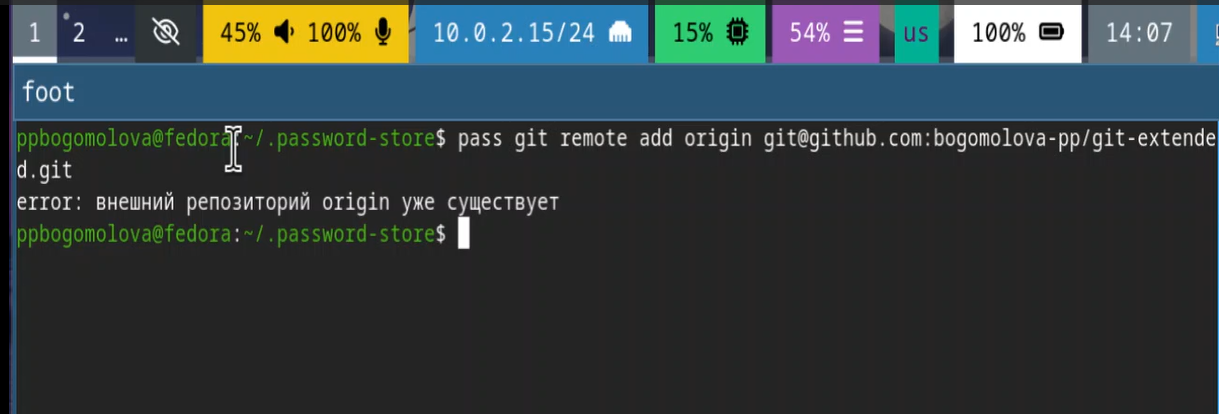
\includegraphics[width=0.5\linewidth,height=\textheight,keepaspectratio]{image/38.png}

}

\caption{\label{fig-008}Рисунок 8 --- Задание адреса репозитория}

\end{figure}%
\end{frame}

\begin{frame}{Синхронизация}
\phantomsection\label{ux441ux438ux43dux445ux440ux43eux43dux438ux437ux430ux446ux438ux44f}
\begin{figure}

\centering{


\includegraphics[width=0.5\linewidth,height=\textheight,keepaspectratio]{image/8.png}

}

\caption{\label{fig-009}Рисунок 9 --- Синхронизация}

\end{figure}%
\end{frame}

\begin{frame}{Синхронизация}
\phantomsection\label{ux441ux438ux43dux445ux440ux43eux43dux438ux437ux430ux446ux438ux44f-1}
\begin{figure}

\centering{


\includegraphics[width=0.5\linewidth,height=\textheight,keepaspectratio]{image/9.png}

}

\caption{\label{fig-010}Рисунок 10 --- Синхронизация}

\end{figure}%
\end{frame}

\begin{frame}{Прямые изменения}
\phantomsection\label{ux43fux440ux44fux43cux44bux435-ux438ux437ux43cux435ux43dux435ux43dux438ux44f}
\begin{figure}

\centering{


\includegraphics[width=0.5\linewidth,height=\textheight,keepaspectratio]{image/10.png}

}

\caption{\label{fig-011}Рисунок 11 --- Прямые изменения}

\end{figure}%
\end{frame}

\begin{frame}{Проверка статуса синхронизации}
\phantomsection\label{ux43fux440ux43eux432ux435ux440ux43aux430-ux441ux442ux430ux442ux443ux441ux430-ux441ux438ux43dux445ux440ux43eux43dux438ux437ux430ux446ux438ux438}
\begin{figure}

\centering{


\includegraphics[width=0.5\linewidth,height=\textheight,keepaspectratio]{image/11.png}

}

\caption{\label{fig-012}Рисунок 12 --- Проверка статуса синхронизации}

\end{figure}%
\end{frame}

\begin{frame}{Установка расширения browserpass}
\phantomsection\label{ux443ux441ux442ux430ux43dux43eux432ux43aux430-ux440ux430ux441ux448ux438ux440ux435ux43dux438ux44f-browserpass}
\begin{figure}

\centering{


\includegraphics[width=0.5\linewidth,height=\textheight,keepaspectratio]{image/12.png}

}

\caption{\label{fig-013}Рисунок 13 --- Установка расширения browserpass}

\end{figure}%
\end{frame}

\begin{frame}{Подключение репозитория browserpass}
\phantomsection\label{ux43fux43eux434ux43aux43bux44eux447ux435ux43dux438ux435-ux440ux435ux43fux43eux437ux438ux442ux43eux440ux438ux44f-browserpass}
\begin{figure}

\centering{


\includegraphics[width=0.5\linewidth,height=\textheight,keepaspectratio]{image/13.png}

}

\caption{\label{fig-014}Рисунок 14 --- Подключение репозитория
browserpass}

\end{figure}%
\end{frame}

\begin{frame}{Установка browserpass}
\phantomsection\label{ux443ux441ux442ux430ux43dux43eux432ux43aux430-browserpass}
\begin{figure}

\centering{


\includegraphics[width=0.5\linewidth,height=\textheight,keepaspectratio]{image/14.png}

}

\caption{\label{fig-015}Рисунок 15 --- Установка browserpass}

\end{figure}%
\end{frame}

\begin{frame}{Установка browserpass}
\phantomsection\label{ux443ux441ux442ux430ux43dux43eux432ux43aux430-browserpass-1}
\begin{figure}

\centering{


\includegraphics[width=0.5\linewidth,height=\textheight,keepaspectratio]{image/15.png}

}

\caption{\label{fig-016}Рисунок 16 --- Установка browserpass}

\end{figure}%
\end{frame}

\begin{frame}{Создание нового пароля}
\phantomsection\label{ux441ux43eux437ux434ux430ux43dux438ux435-ux43dux43eux432ux43eux433ux43e-ux43fux430ux440ux43eux43bux44f}
\begin{figure}

\centering{


\includegraphics[width=0.5\linewidth,height=\textheight,keepaspectratio]{image/16.png}

}

\caption{\label{fig-017}Рисунок 17 --- Создание нового пароля}

\end{figure}%
\end{frame}

\begin{frame}{Просмотр сохраненного пароля}
\phantomsection\label{ux43fux440ux43eux441ux43cux43eux442ux440-ux441ux43eux445ux440ux430ux43dux435ux43dux43dux43eux433ux43e-ux43fux430ux440ux43eux43bux44f}
\begin{figure}

\centering{


\includegraphics[width=0.5\linewidth,height=\textheight,keepaspectratio]{image/17.png}

}

\caption{\label{fig-018}Рисунок 18 --- Просмотр сохраненного пароля}

\end{figure}%
\end{frame}

\begin{frame}{Установка дополнительного ПО}
\phantomsection\label{ux443ux441ux442ux430ux43dux43eux432ux43aux430-ux434ux43eux43fux43eux43bux43dux438ux442ux435ux43bux44cux43dux43eux433ux43e-ux43fux43e}
\begin{figure}

\centering{


\includegraphics[width=0.5\linewidth,height=\textheight,keepaspectratio]{image/18.png}

}

\caption{\label{fig-019}Рисунок 19 --- Установка дополнительного ПО}

\end{figure}%
\end{frame}

\begin{frame}{Установка дополнительного ПО}
\phantomsection\label{ux443ux441ux442ux430ux43dux43eux432ux43aux430-ux434ux43eux43fux43eux43bux43dux438ux442ux435ux43bux44cux43dux43eux433ux43e-ux43fux43e-1}
\begin{figure}

\centering{


\includegraphics[width=0.5\linewidth,height=\textheight,keepaspectratio]{image/19.png}

}

\caption{\label{fig-020}Рисунок 20 --- Установка дополнительного ПО}

\end{figure}%
\end{frame}

\begin{frame}{Генерация нового пароля}
\phantomsection\label{ux433ux435ux43dux435ux440ux430ux446ux438ux44f-ux43dux43eux432ux43eux433ux43e-ux43fux430ux440ux43eux43bux44f}
\begin{figure}

\centering{


\includegraphics[width=0.5\linewidth,height=\textheight,keepaspectratio]{image/20.png}

}

\caption{\label{fig-021}Рисунок 21 --- Генерация нового пароля}

\end{figure}%
\end{frame}

\begin{frame}{Подключение стороннего репозитория}
\phantomsection\label{ux43fux43eux434ux43aux43bux44eux447ux435ux43dux438ux435-ux441ux442ux43eux440ux43eux43dux43dux435ux433ux43e-ux440ux435ux43fux43eux437ux438ux442ux43eux440ux438ux44f}
\begin{figure}

\centering{


\includegraphics[width=0.5\linewidth,height=\textheight,keepaspectratio]{image/21.png}

}

\caption{\label{fig-022}Рисунок 22 --- Подключение стороннего
репозитория}

\end{figure}%
\end{frame}

\begin{frame}{Поиск пакета iosevka}
\phantomsection\label{ux43fux43eux438ux441ux43a-ux43fux430ux43aux435ux442ux430-iosevka}
\begin{figure}

\centering{


\includegraphics[width=0.5\linewidth,height=\textheight,keepaspectratio]{image/22.png}

}

\caption{\label{fig-023}Рисунок 23 --- Поиск пакета iosevka}

\end{figure}%
\end{frame}

\begin{frame}{Поиск пакета iosevka}
\phantomsection\label{ux43fux43eux438ux441ux43a-ux43fux430ux43aux435ux442ux430-iosevka-1}
\begin{figure}

\centering{


\includegraphics[width=0.5\linewidth,height=\textheight,keepaspectratio]{image/23.png}

}

\caption{\label{fig-024}Рисунок 24 --- Поиск пакета iosevka}

\end{figure}%
\end{frame}

\begin{frame}{Успешная установка iosevka}
\phantomsection\label{ux443ux441ux43fux435ux448ux43dux430ux44f-ux443ux441ux442ux430ux43dux43eux432ux43aux430-iosevka}
\begin{figure}

\centering{


\includegraphics[width=0.5\linewidth,height=\textheight,keepaspectratio]{image/24.png}

}

\caption{\label{fig-025}Рисунок 25 --- Успешная установка iosevka}

\end{figure}%
\end{frame}

\begin{frame}{Установка бинарного файла}
\phantomsection\label{ux443ux441ux442ux430ux43dux43eux432ux43aux430-ux431ux438ux43dux430ux440ux43dux43eux433ux43e-ux444ux430ux439ux43bux430}
\begin{figure}

\centering{


\includegraphics[width=0.5\linewidth,height=\textheight,keepaspectratio]{image/25.png}

}

\caption{\label{fig-026}Рисунок 26 --- Установка бинарного файла}

\end{figure}%
\end{frame}

\begin{frame}{Создание репозитория dotfiles}
\phantomsection\label{ux441ux43eux437ux434ux430ux43dux438ux435-ux440ux435ux43fux43eux437ux438ux442ux43eux440ux438ux44f-dotfiles}
\begin{figure}

\centering{


\includegraphics[width=0.5\linewidth,height=\textheight,keepaspectratio]{image/26.png}

}

\caption{\label{fig-027}Рисунок 27 --- Создание репозитория dotfiles}

\end{figure}%
\end{frame}

\begin{frame}{Инициализация chezmoi}
\phantomsection\label{ux438ux43dux438ux446ux438ux430ux43bux438ux437ux430ux446ux438ux44f-chezmoi}
\begin{figure}

\centering{


\includegraphics[width=0.5\linewidth,height=\textheight,keepaspectratio]{image/27.png}

}

\caption{\label{fig-028}Рисунок 28 --- Инициализация chezmoi}

\end{figure}%
\end{frame}

\begin{frame}{Проверка изменений}
\phantomsection\label{ux43fux440ux43eux432ux435ux440ux43aux430-ux438ux437ux43cux435ux43dux435ux43dux438ux439}
\begin{figure}

\centering{

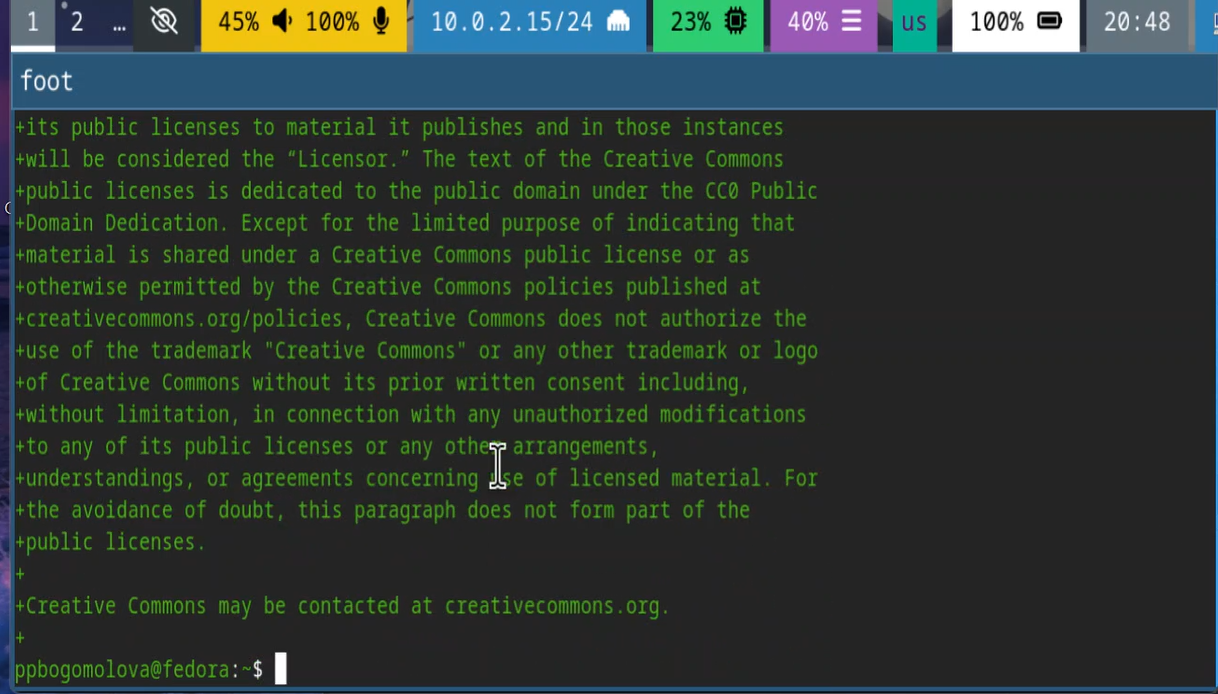
\includegraphics[width=0.5\linewidth,height=\textheight,keepaspectratio]{image/39.png}

}

\caption{\label{fig-029}Рисунок 29 --- Проверка изменений}

\end{figure}%
\end{frame}

\begin{frame}{Применение изменений}
\phantomsection\label{ux43fux440ux438ux43cux435ux43dux435ux43dux438ux435-ux438ux437ux43cux435ux43dux435ux43dux438ux439}
\begin{figure}

\centering{

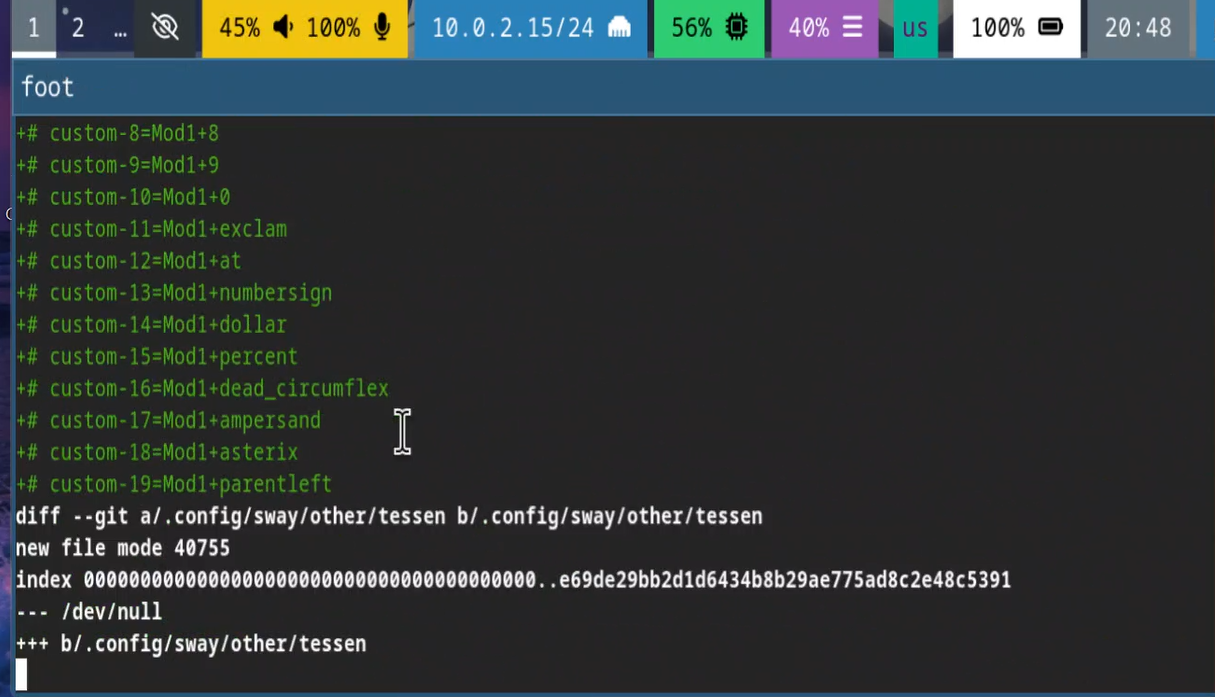
\includegraphics[width=0.5\linewidth,height=\textheight,keepaspectratio]{image/40.png}

}

\caption{\label{fig-030}Рисунок 30 --- Применение изменений}

\end{figure}%
\end{frame}

\begin{frame}{Инициализация chezmoi на второй машине}
\phantomsection\label{ux438ux43dux438ux446ux438ux430ux43bux438ux437ux430ux446ux438ux44f-chezmoi-ux43dux430-ux432ux442ux43eux440ux43eux439-ux43cux430ux448ux438ux43dux435}
\begin{figure}

\centering{

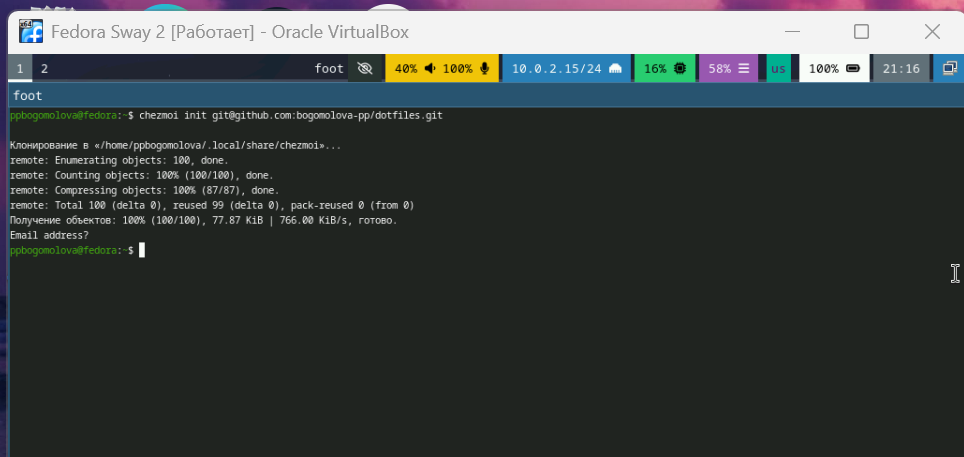
\includegraphics[width=0.5\linewidth,height=\textheight,keepaspectratio]{image/29.png}

}

\caption{\label{fig-031}Рисунок 31 --- Инициализация chezmoi на второй
машине}

\end{figure}%
\end{frame}

\begin{frame}{Проверка изменений на второй машине}
\phantomsection\label{ux43fux440ux43eux432ux435ux440ux43aux430-ux438ux437ux43cux435ux43dux435ux43dux438ux439-ux43dux430-ux432ux442ux43eux440ux43eux439-ux43cux430ux448ux438ux43dux435}
\begin{figure}

\centering{

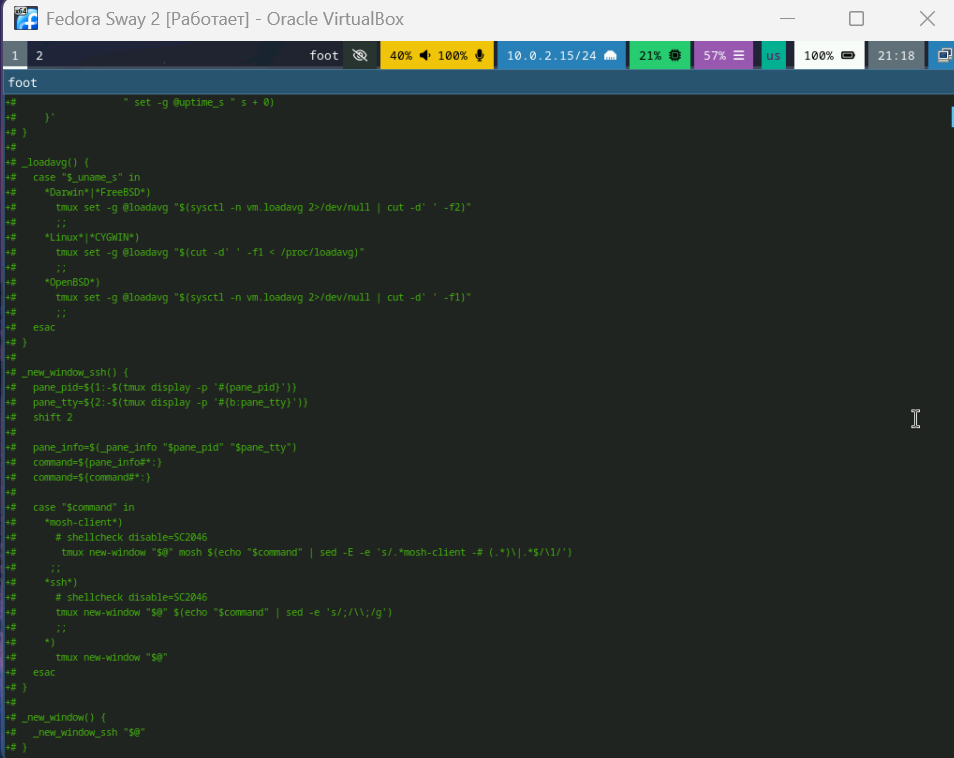
\includegraphics[width=0.5\linewidth,height=\textheight,keepaspectratio]{image/30.png}

}

\caption{\label{fig-032}Рисунок 32 --- Проверка изменений на второй
машине}

\end{figure}%
\end{frame}

\begin{frame}{Применение изменений}
\phantomsection\label{ux43fux440ux438ux43cux435ux43dux435ux43dux438ux435-ux438ux437ux43cux435ux43dux435ux43dux438ux439-1}
\begin{figure}

\centering{

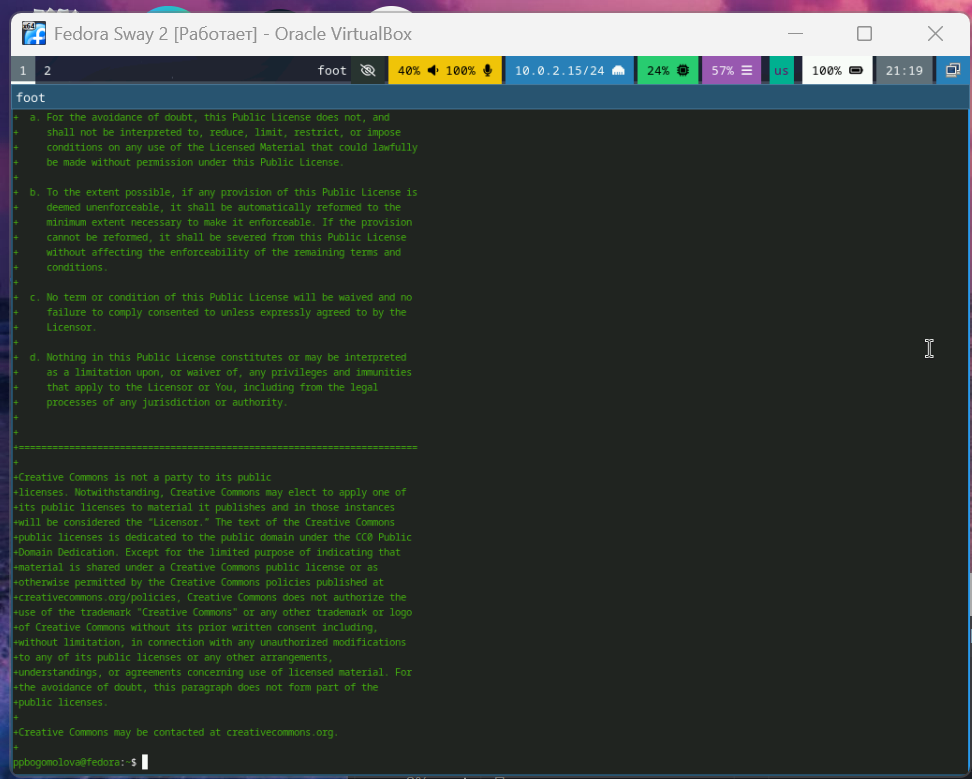
\includegraphics[width=0.5\linewidth,height=\textheight,keepaspectratio]{image/31.png}

}

\caption{\label{fig-033}Рисунок 33 --- Применение изменений}

\end{figure}%
\end{frame}

\begin{frame}{Получение последних изменений}
\phantomsection\label{ux43fux43eux43bux443ux447ux435ux43dux438ux435-ux43fux43eux441ux43bux435ux434ux43dux438ux445-ux438ux437ux43cux435ux43dux435ux43dux438ux439}
\begin{figure}

\centering{

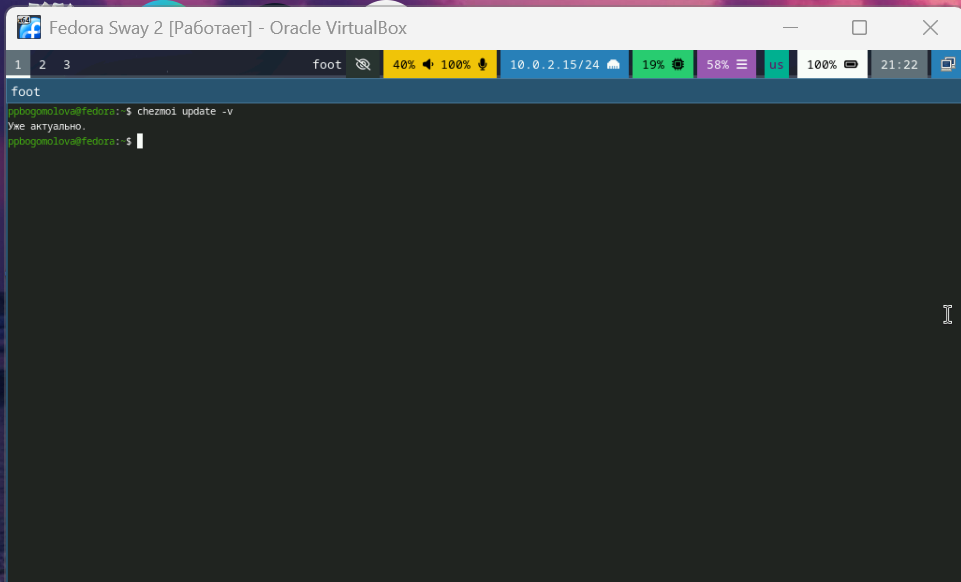
\includegraphics[width=0.5\linewidth,height=\textheight,keepaspectratio]{image/32.png}

}

\caption{\label{fig-034}Рисунок 34 --- Получение последних изменений}

\end{figure}%
\end{frame}

\begin{frame}{Получение последних изменений}
\phantomsection\label{ux43fux43eux43bux443ux447ux435ux43dux438ux435-ux43fux43eux441ux43bux435ux434ux43dux438ux445-ux438ux437ux43cux435ux43dux435ux43dux438ux439-1}
\begin{figure}

\centering{

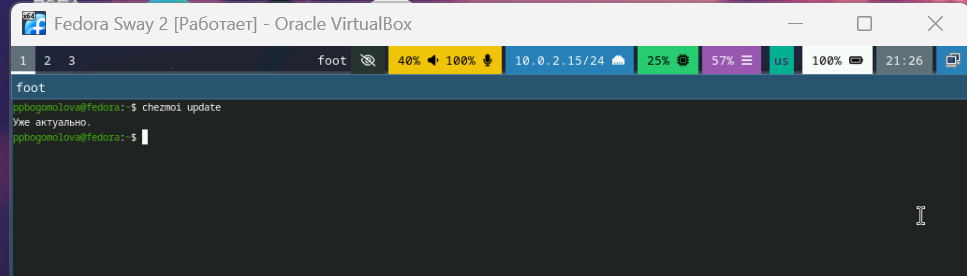
\includegraphics[width=0.5\linewidth,height=\textheight,keepaspectratio]{image/33.png}

}

\caption{\label{fig-035}Рисунок 35 --- Получение последних изменений}

\end{figure}%
\end{frame}

\begin{frame}{Настройка новой машины}
\phantomsection\label{ux43dux430ux441ux442ux440ux43eux439ux43aux430-ux43dux43eux432ux43eux439-ux43cux430ux448ux438ux43dux44b}
\begin{figure}

\centering{

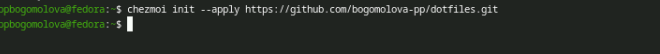
\includegraphics[width=0.5\linewidth,height=\textheight,keepaspectratio]{image/34.png}

}

\caption{\label{fig-036}Рисунок 36 --- Установка dotfiles}

\end{figure}%
\end{frame}

\begin{frame}{Команда chezmoi apply}
\phantomsection\label{ux43aux43eux43cux430ux43dux434ux430-chezmoi-apply}
\begin{figure}

\centering{

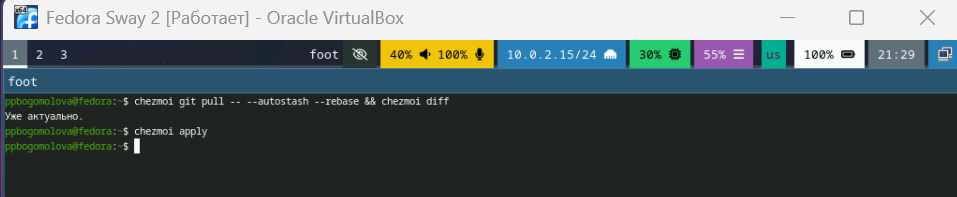
\includegraphics[width=0.5\linewidth,height=\textheight,keepaspectratio]{image/35.png}

}

\caption{\label{fig-037}Рисунок 37 --- Выполнение chezmoi apply}

\end{figure}%
\end{frame}

\begin{frame}{Конфигурационный файл chezmoi}
\phantomsection\label{ux43aux43eux43dux444ux438ux433ux443ux440ux430ux446ux438ux43eux43dux43dux44bux439-ux444ux430ux439ux43b-chezmoi}
\begin{figure}

\centering{

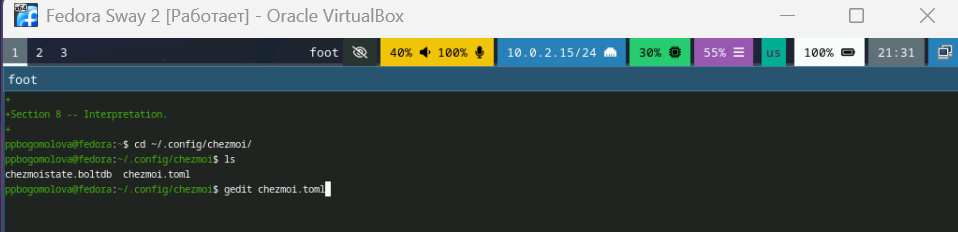
\includegraphics[width=0.5\linewidth,height=\textheight,keepaspectratio]{image/36.png}

}

\caption{\label{fig-038}Рисунок 38 --- Открытие конфигурационного файла}

\end{figure}%
\end{frame}

\begin{frame}{Отредактированный конфигурационный файл}
\phantomsection\label{ux43eux442ux440ux435ux434ux430ux43aux442ux438ux440ux43eux432ux430ux43dux43dux44bux439-ux43aux43eux43dux444ux438ux433ux443ux440ux430ux446ux438ux43eux43dux43dux44bux439-ux444ux430ux439ux43b}
\begin{figure}

\centering{

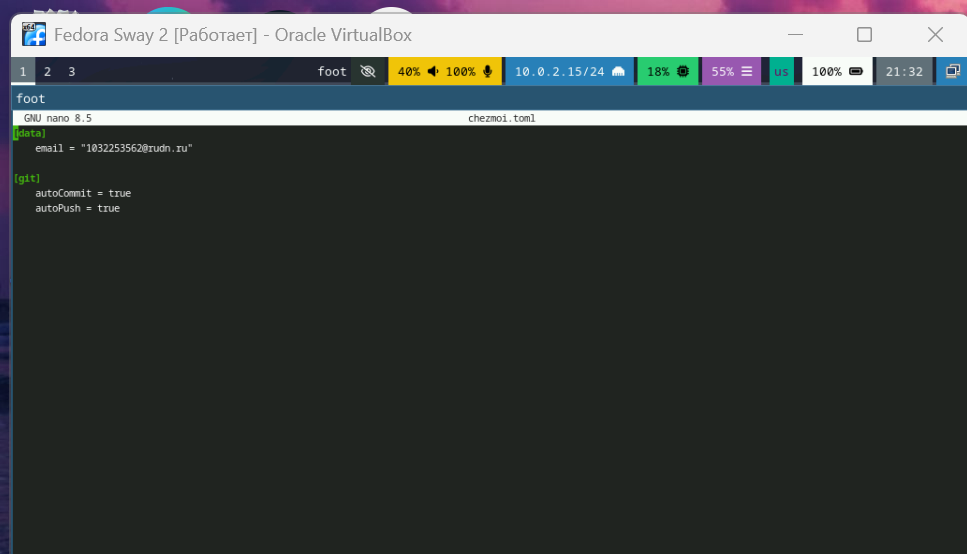
\includegraphics[width=0.5\linewidth,height=\textheight,keepaspectratio]{image/37.png}

}

\caption{\label{fig-039}Рисунок 39 --- Отредактированный
конфигурационный файл}

\end{figure}%
\end{frame}

\begin{frame}{Выводы}
\phantomsection\label{ux432ux44bux432ux43eux434ux44b}
Установлены менеджеры паролей pass и gopass.\\
Настроена интеграция с браузером.\\
Освоена синхронизация конфигураций между машинами.
\end{frame}




\end{document}
